% Options for packages loaded elsewhere
\PassOptionsToPackage{unicode}{hyperref}
\PassOptionsToPackage{hyphens}{url}
\PassOptionsToPackage{dvipsnames,svgnames,x11names}{xcolor}
%
\documentclass[
  letterpaper,
  DIV=11,
  numbers=noendperiod]{scrartcl}

\usepackage{amsmath,amssymb}
\usepackage{iftex}
\ifPDFTeX
  \usepackage[T1]{fontenc}
  \usepackage[utf8]{inputenc}
  \usepackage{textcomp} % provide euro and other symbols
\else % if luatex or xetex
  \usepackage{unicode-math}
  \defaultfontfeatures{Scale=MatchLowercase}
  \defaultfontfeatures[\rmfamily]{Ligatures=TeX,Scale=1}
\fi
\usepackage{lmodern}
\ifPDFTeX\else  
    % xetex/luatex font selection
\fi
% Use upquote if available, for straight quotes in verbatim environments
\IfFileExists{upquote.sty}{\usepackage{upquote}}{}
\IfFileExists{microtype.sty}{% use microtype if available
  \usepackage[]{microtype}
  \UseMicrotypeSet[protrusion]{basicmath} % disable protrusion for tt fonts
}{}
\makeatletter
\@ifundefined{KOMAClassName}{% if non-KOMA class
  \IfFileExists{parskip.sty}{%
    \usepackage{parskip}
  }{% else
    \setlength{\parindent}{0pt}
    \setlength{\parskip}{6pt plus 2pt minus 1pt}}
}{% if KOMA class
  \KOMAoptions{parskip=half}}
\makeatother
\usepackage{xcolor}
\setlength{\emergencystretch}{3em} % prevent overfull lines
\setcounter{secnumdepth}{-\maxdimen} % remove section numbering
% Make \paragraph and \subparagraph free-standing
\makeatletter
\ifx\paragraph\undefined\else
  \let\oldparagraph\paragraph
  \renewcommand{\paragraph}{
    \@ifstar
      \xxxParagraphStar
      \xxxParagraphNoStar
  }
  \newcommand{\xxxParagraphStar}[1]{\oldparagraph*{#1}\mbox{}}
  \newcommand{\xxxParagraphNoStar}[1]{\oldparagraph{#1}\mbox{}}
\fi
\ifx\subparagraph\undefined\else
  \let\oldsubparagraph\subparagraph
  \renewcommand{\subparagraph}{
    \@ifstar
      \xxxSubParagraphStar
      \xxxSubParagraphNoStar
  }
  \newcommand{\xxxSubParagraphStar}[1]{\oldsubparagraph*{#1}\mbox{}}
  \newcommand{\xxxSubParagraphNoStar}[1]{\oldsubparagraph{#1}\mbox{}}
\fi
\makeatother

\usepackage{color}
\usepackage{fancyvrb}
\newcommand{\VerbBar}{|}
\newcommand{\VERB}{\Verb[commandchars=\\\{\}]}
\DefineVerbatimEnvironment{Highlighting}{Verbatim}{commandchars=\\\{\}}
% Add ',fontsize=\small' for more characters per line
\usepackage{framed}
\definecolor{shadecolor}{RGB}{241,243,245}
\newenvironment{Shaded}{\begin{snugshade}}{\end{snugshade}}
\newcommand{\AlertTok}[1]{\textcolor[rgb]{0.68,0.00,0.00}{#1}}
\newcommand{\AnnotationTok}[1]{\textcolor[rgb]{0.37,0.37,0.37}{#1}}
\newcommand{\AttributeTok}[1]{\textcolor[rgb]{0.40,0.45,0.13}{#1}}
\newcommand{\BaseNTok}[1]{\textcolor[rgb]{0.68,0.00,0.00}{#1}}
\newcommand{\BuiltInTok}[1]{\textcolor[rgb]{0.00,0.23,0.31}{#1}}
\newcommand{\CharTok}[1]{\textcolor[rgb]{0.13,0.47,0.30}{#1}}
\newcommand{\CommentTok}[1]{\textcolor[rgb]{0.37,0.37,0.37}{#1}}
\newcommand{\CommentVarTok}[1]{\textcolor[rgb]{0.37,0.37,0.37}{\textit{#1}}}
\newcommand{\ConstantTok}[1]{\textcolor[rgb]{0.56,0.35,0.01}{#1}}
\newcommand{\ControlFlowTok}[1]{\textcolor[rgb]{0.00,0.23,0.31}{\textbf{#1}}}
\newcommand{\DataTypeTok}[1]{\textcolor[rgb]{0.68,0.00,0.00}{#1}}
\newcommand{\DecValTok}[1]{\textcolor[rgb]{0.68,0.00,0.00}{#1}}
\newcommand{\DocumentationTok}[1]{\textcolor[rgb]{0.37,0.37,0.37}{\textit{#1}}}
\newcommand{\ErrorTok}[1]{\textcolor[rgb]{0.68,0.00,0.00}{#1}}
\newcommand{\ExtensionTok}[1]{\textcolor[rgb]{0.00,0.23,0.31}{#1}}
\newcommand{\FloatTok}[1]{\textcolor[rgb]{0.68,0.00,0.00}{#1}}
\newcommand{\FunctionTok}[1]{\textcolor[rgb]{0.28,0.35,0.67}{#1}}
\newcommand{\ImportTok}[1]{\textcolor[rgb]{0.00,0.46,0.62}{#1}}
\newcommand{\InformationTok}[1]{\textcolor[rgb]{0.37,0.37,0.37}{#1}}
\newcommand{\KeywordTok}[1]{\textcolor[rgb]{0.00,0.23,0.31}{\textbf{#1}}}
\newcommand{\NormalTok}[1]{\textcolor[rgb]{0.00,0.23,0.31}{#1}}
\newcommand{\OperatorTok}[1]{\textcolor[rgb]{0.37,0.37,0.37}{#1}}
\newcommand{\OtherTok}[1]{\textcolor[rgb]{0.00,0.23,0.31}{#1}}
\newcommand{\PreprocessorTok}[1]{\textcolor[rgb]{0.68,0.00,0.00}{#1}}
\newcommand{\RegionMarkerTok}[1]{\textcolor[rgb]{0.00,0.23,0.31}{#1}}
\newcommand{\SpecialCharTok}[1]{\textcolor[rgb]{0.37,0.37,0.37}{#1}}
\newcommand{\SpecialStringTok}[1]{\textcolor[rgb]{0.13,0.47,0.30}{#1}}
\newcommand{\StringTok}[1]{\textcolor[rgb]{0.13,0.47,0.30}{#1}}
\newcommand{\VariableTok}[1]{\textcolor[rgb]{0.07,0.07,0.07}{#1}}
\newcommand{\VerbatimStringTok}[1]{\textcolor[rgb]{0.13,0.47,0.30}{#1}}
\newcommand{\WarningTok}[1]{\textcolor[rgb]{0.37,0.37,0.37}{\textit{#1}}}

\providecommand{\tightlist}{%
  \setlength{\itemsep}{0pt}\setlength{\parskip}{0pt}}\usepackage{longtable,booktabs,array}
\usepackage{calc} % for calculating minipage widths
% Correct order of tables after \paragraph or \subparagraph
\usepackage{etoolbox}
\makeatletter
\patchcmd\longtable{\par}{\if@noskipsec\mbox{}\fi\par}{}{}
\makeatother
% Allow footnotes in longtable head/foot
\IfFileExists{footnotehyper.sty}{\usepackage{footnotehyper}}{\usepackage{footnote}}
\makesavenoteenv{longtable}
\usepackage{graphicx}
\makeatletter
\def\maxwidth{\ifdim\Gin@nat@width>\linewidth\linewidth\else\Gin@nat@width\fi}
\def\maxheight{\ifdim\Gin@nat@height>\textheight\textheight\else\Gin@nat@height\fi}
\makeatother
% Scale images if necessary, so that they will not overflow the page
% margins by default, and it is still possible to overwrite the defaults
% using explicit options in \includegraphics[width, height, ...]{}
\setkeys{Gin}{width=\maxwidth,height=\maxheight,keepaspectratio}
% Set default figure placement to htbp
\makeatletter
\def\fps@figure{htbp}
\makeatother

\usepackage{booktabs}
\usepackage{longtable}
\usepackage{array}
\usepackage{multirow}
\usepackage{wrapfig}
\usepackage{float}
\usepackage{colortbl}
\usepackage{pdflscape}
\usepackage{tabu}
\usepackage{threeparttable}
\usepackage{threeparttablex}
\usepackage[normalem]{ulem}
\usepackage{makecell}
\usepackage{xcolor}
\KOMAoption{captions}{tableheading}
\makeatletter
\@ifpackageloaded{caption}{}{\usepackage{caption}}
\AtBeginDocument{%
\ifdefined\contentsname
  \renewcommand*\contentsname{Table of contents}
\else
  \newcommand\contentsname{Table of contents}
\fi
\ifdefined\listfigurename
  \renewcommand*\listfigurename{List of Figures}
\else
  \newcommand\listfigurename{List of Figures}
\fi
\ifdefined\listtablename
  \renewcommand*\listtablename{List of Tables}
\else
  \newcommand\listtablename{List of Tables}
\fi
\ifdefined\figurename
  \renewcommand*\figurename{Figure}
\else
  \newcommand\figurename{Figure}
\fi
\ifdefined\tablename
  \renewcommand*\tablename{Table}
\else
  \newcommand\tablename{Table}
\fi
}
\@ifpackageloaded{float}{}{\usepackage{float}}
\floatstyle{ruled}
\@ifundefined{c@chapter}{\newfloat{codelisting}{h}{lop}}{\newfloat{codelisting}{h}{lop}[chapter]}
\floatname{codelisting}{Listing}
\newcommand*\listoflistings{\listof{codelisting}{List of Listings}}
\makeatother
\makeatletter
\makeatother
\makeatletter
\@ifpackageloaded{caption}{}{\usepackage{caption}}
\@ifpackageloaded{subcaption}{}{\usepackage{subcaption}}
\makeatother

\ifLuaTeX
  \usepackage{selnolig}  % disable illegal ligatures
\fi
\usepackage{bookmark}

\IfFileExists{xurl.sty}{\usepackage{xurl}}{} % add URL line breaks if available
\urlstyle{same} % disable monospaced font for URLs
\hypersetup{
  pdftitle={Untitled},
  colorlinks=true,
  linkcolor={blue},
  filecolor={Maroon},
  citecolor={Blue},
  urlcolor={Blue},
  pdfcreator={LaTeX via pandoc}}


\title{Untitled}
\author{}
\date{}

\begin{document}
\maketitle


\subsection{Análisis Estadistico}\label{anuxe1lisis-estadistico}

La base de datos ya se encuentra en formato en tidy, recordemos que el
formato tidy fue popularizado por el autor Hadley Wickham, donde indican
que cada variable debe tener su propia columna y cada observación su
propia fila. Nuestra base de datos cumple con estar en formato tidy.

Vamos a llamar a nuestra base de datos, la cual vamos a utilizar durante
el trabajo.

\begin{Shaded}
\begin{Highlighting}[]
\FunctionTok{library}\NormalTok{(readr)}
\FunctionTok{library}\NormalTok{(tidyverse)}
\end{Highlighting}
\end{Shaded}

\begin{verbatim}
-- Attaching core tidyverse packages ------------------------ tidyverse 2.0.0 --
v dplyr     1.1.4     v purrr     1.0.2
v forcats   1.0.0     v stringr   1.5.1
v ggplot2   3.5.1     v tibble    3.2.1
v lubridate 1.9.3     v tidyr     1.3.1
-- Conflicts ------------------------------------------ tidyverse_conflicts() --
x dplyr::filter() masks stats::filter()
x dplyr::lag()    masks stats::lag()
i Use the conflicted package (<http://conflicted.r-lib.org/>) to force all conflicts to become errors
\end{verbatim}

\begin{Shaded}
\begin{Highlighting}[]
\NormalTok{data\_accidentes }\OtherTok{\textless{}{-}}  \FunctionTok{read.csv}\NormalTok{(}\StringTok{"../data/clean\_data.csv"}\NormalTok{)}

\NormalTok{data\_accidentes }\OtherTok{\textless{}{-}}\NormalTok{ data\_accidentes }\SpecialCharTok{\%\textgreater{}\%} 
  \FunctionTok{select}\NormalTok{(}\SpecialCharTok{{-}}\NormalTok{X) }\SpecialCharTok{\%\textgreater{}\%}
  \FunctionTok{select}\NormalTok{(}\SpecialCharTok{{-}}\NormalTok{pedestrian) }\SpecialCharTok{\%\textgreater{}\%}
  \FunctionTok{select}\NormalTok{(}\SpecialCharTok{{-}}\NormalTok{flatHill) }\SpecialCharTok{\%\textgreater{}\%}
  \FunctionTok{select}\NormalTok{(}\SpecialCharTok{{-}}\NormalTok{tlaId) }\SpecialCharTok{\%\textgreater{}\%}
  \FunctionTok{select}\NormalTok{(}\SpecialCharTok{{-}}\NormalTok{trafficControl)}

\NormalTok{data\_accidentes}\SpecialCharTok{$}\NormalTok{holiday }\OtherTok{\textless{}{-}} \FunctionTok{ifelse}\NormalTok{(}\FunctionTok{is.na}\NormalTok{(data\_accidentes}\SpecialCharTok{$}\NormalTok{holiday) }\SpecialCharTok{|}\NormalTok{ data\_accidentes}\SpecialCharTok{$}\NormalTok{holiday }\SpecialCharTok{==} \StringTok{""}\NormalTok{, }\StringTok{"No festivo"}\NormalTok{, data\_accidentes}\SpecialCharTok{$}\NormalTok{holiday)}
\end{Highlighting}
\end{Shaded}

\begin{Shaded}
\begin{Highlighting}[]
\FunctionTok{head}\NormalTok{(data\_accidentes)}
\end{Highlighting}
\end{Shaded}

\begin{verbatim}
  advisorySpeed    crashSeverity fatalCount    holiday      light
1            NA      Minor Crash          0 No festivo   Overcast
2            NA Non-Injury Crash          0 No festivo Bright sun
3            NA Non-Injury Crash          0 No festivo Bright sun
4            NA Non-Injury Crash          0 No festivo       Dark
5            NA Non-Injury Crash          0 No festivo   Overcast
6            40 Non-Injury Crash          0 No festivo   Twilight
  minorInjuryCount roadSurface seriousInjuryCount speedLimit    weather
1                1      Sealed                  0         50 Light rain
2                0      Sealed                  0         50       Fine
3                0      Sealed                  0         50       Fine
4                0      Sealed                  0         50 Light rain
5                0      Sealed                  0         50       Fine
6                0      Sealed                  0         50 Light rain
\end{verbatim}

Antes de aplicar cualquier gráfico o análisis de datos a nuestra base de
datos, es importante eliminar las variables que no aportan al estudio,
por ello, vamos a eliminar los valores NA que vengan en nuestra base de
datos y columnas que no sean de nuestro interés.

\begin{Shaded}
\begin{Highlighting}[]
\FunctionTok{library}\NormalTok{(dplyr)}
  
\NormalTok{data\_limpia }\OtherTok{\textless{}{-}} \FunctionTok{na.omit}\NormalTok{(data\_accidentes)}

\NormalTok{data }\OtherTok{\textless{}{-}}\NormalTok{ data\_limpia}

\FunctionTok{colnames}\NormalTok{(data) }\OtherTok{\textless{}{-}} \FunctionTok{c}\NormalTok{(}\StringTok{"velocidad\_recomendada"}\NormalTok{, }\StringTok{"severidad"}\NormalTok{, }\StringTok{"fatales"}\NormalTok{ ,}\StringTok{"festivos"}\NormalTok{, }\StringTok{"iluminación"}\NormalTok{, }\StringTok{"lesiones\_menores"}\NormalTok{, }\StringTok{"carretera"}\NormalTok{, }\StringTok{"lesiones\_graves"}\NormalTok{, }\StringTok{"limite\_velocidad"}\NormalTok{, }\StringTok{"clima"}\NormalTok{)}


\NormalTok{data }\OtherTok{\textless{}{-}}\NormalTok{ data }\SpecialCharTok{\%\textgreater{}\%}
  \FunctionTok{mutate}\NormalTok{(}\AttributeTok{clima =} \FunctionTok{case\_when}\NormalTok{(}
\NormalTok{    clima }\SpecialCharTok{\%in\%} \FunctionTok{c}\NormalTok{(}\StringTok{"Fine"}\NormalTok{, }\StringTok{"Fine \& Frost"}\NormalTok{, }\StringTok{"Fine \& Strong wind"}\NormalTok{) }\SpecialCharTok{\textasciitilde{}} \StringTok{"Buen clima"}\NormalTok{,}
\NormalTok{    clima }\SpecialCharTok{\%in\%} \FunctionTok{c}\NormalTok{(}\StringTok{"Light rain"}\NormalTok{, }\StringTok{"Light rain \& Frost"}\NormalTok{, }\StringTok{"Light rain \& Strong wind"}\NormalTok{) }\SpecialCharTok{\textasciitilde{}} \StringTok{"Lluvia ligera"}\NormalTok{,}
\NormalTok{    clima }\SpecialCharTok{\%in\%} \FunctionTok{c}\NormalTok{(}\StringTok{"Heavy rain"}\NormalTok{, }\StringTok{"Heavy rain \& Frost"}\NormalTok{, }\StringTok{"Heavy rain \& Strong wind"}\NormalTok{) }\SpecialCharTok{\textasciitilde{}} \StringTok{"Lluvia intensa"}\NormalTok{,}
\NormalTok{    clima }\SpecialCharTok{\%in\%} \FunctionTok{c}\NormalTok{(}\StringTok{"Snow"}\NormalTok{, }\StringTok{"Snow \& Frost"}\NormalTok{, }\StringTok{"Snow \& Strong wind"}\NormalTok{) }\SpecialCharTok{\textasciitilde{}} \StringTok{"Nieve"}\NormalTok{,}
\NormalTok{    clima }\SpecialCharTok{\%in\%} \FunctionTok{c}\NormalTok{(}\StringTok{"Hail or Sleet"}\NormalTok{, }\StringTok{"Hail or Sleet \& Frost"}\NormalTok{, }\StringTok{"Hail or Sleet \& Strong wind"}\NormalTok{) }\SpecialCharTok{\textasciitilde{}} \StringTok{"Granizo"}\NormalTok{,}
\NormalTok{    clima }\SpecialCharTok{\%in\%} \FunctionTok{c}\NormalTok{(}\StringTok{"Mist or Fog"}\NormalTok{, }\StringTok{"Mist or Fog \& Frost"}\NormalTok{, }\StringTok{"Mist or Fog \& Strong wind"}\NormalTok{) }\SpecialCharTok{\textasciitilde{}} \StringTok{"Niebla"}
\NormalTok{  ))}


\NormalTok{data }\OtherTok{\textless{}{-}}\NormalTok{ data }\SpecialCharTok{\%\textgreater{}\%}
  \FunctionTok{mutate}\NormalTok{(}\AttributeTok{severidad =} \FunctionTok{case\_when}\NormalTok{(}
\NormalTok{    severidad }\SpecialCharTok{\%in\%} \FunctionTok{c}\NormalTok{(}\StringTok{"Non{-}Injury Crash"}\NormalTok{) }\SpecialCharTok{\textasciitilde{}} \StringTok{"Accidente sin lesiones"}\NormalTok{,}
\NormalTok{        severidad }\SpecialCharTok{\%in\%} \FunctionTok{c}\NormalTok{(}\StringTok{"Minor Crash"}\NormalTok{) }\SpecialCharTok{\textasciitilde{}} \StringTok{"Accidente leve"}\NormalTok{,}
\NormalTok{    severidad }\SpecialCharTok{\%in\%} \FunctionTok{c}\NormalTok{(}\StringTok{"Fatal Crash"}\NormalTok{) }\SpecialCharTok{\textasciitilde{}} \StringTok{"Accidente fatal"}\NormalTok{,}
\NormalTok{    severidad }\SpecialCharTok{\%in\%} \FunctionTok{c}\NormalTok{(}\StringTok{"Serious Crash"}\NormalTok{) }\SpecialCharTok{\textasciitilde{}} \StringTok{"Accidente grave"}
\NormalTok{  ))}


\NormalTok{data }\OtherTok{\textless{}{-}}\NormalTok{ data }\SpecialCharTok{\%\textgreater{}\%}
  \FunctionTok{mutate}\NormalTok{(}\AttributeTok{carretera =} \FunctionTok{case\_when}\NormalTok{(}
\NormalTok{    carretera }\SpecialCharTok{\%in\%} \FunctionTok{c}\NormalTok{(}\StringTok{"End of seal"}\NormalTok{) }\SpecialCharTok{\textasciitilde{}} \StringTok{"Final del asfalto"}\NormalTok{,}
\NormalTok{    carretera }\SpecialCharTok{\%in\%} \FunctionTok{c}\NormalTok{(}\StringTok{"Sealed"}\NormalTok{) }\SpecialCharTok{\textasciitilde{}} \StringTok{"Asfalto"}\NormalTok{,}
\NormalTok{    carretera }\SpecialCharTok{\%in\%} \FunctionTok{c}\NormalTok{(}\StringTok{"Unsealed"}\NormalTok{) }\SpecialCharTok{\textasciitilde{}} \StringTok{"Sin Asfalto"}\NormalTok{,}
\NormalTok{  ))}


\NormalTok{data }\OtherTok{\textless{}{-}}\NormalTok{ data }\SpecialCharTok{\%\textgreater{}\%}
  \FunctionTok{mutate}\NormalTok{(iluminación }\OtherTok{=} \FunctionTok{case\_when}\NormalTok{(}
\NormalTok{    iluminación }\SpecialCharTok{\%in\%} \FunctionTok{c}\NormalTok{(}\StringTok{"Bright sun"}\NormalTok{) }\SpecialCharTok{\textasciitilde{}} \StringTok{"Soleado"}\NormalTok{,}
\NormalTok{    iluminación }\SpecialCharTok{\%in\%} \FunctionTok{c}\NormalTok{(}\StringTok{"Overcast"}\NormalTok{) }\SpecialCharTok{\textasciitilde{}} \StringTok{"Nublado"}\NormalTok{,}
\NormalTok{    iluminación }\SpecialCharTok{\%in\%} \FunctionTok{c}\NormalTok{(}\StringTok{"Twilight"}\NormalTok{) }\SpecialCharTok{\textasciitilde{}} \StringTok{"Amanecer o atardecer"}\NormalTok{,}
\NormalTok{    iluminación }\SpecialCharTok{\%in\%} \FunctionTok{c}\NormalTok{(}\StringTok{"Dark"}\NormalTok{) }\SpecialCharTok{\textasciitilde{}} \StringTok{"Oscuro"}\NormalTok{,}
\NormalTok{    iluminación }\SpecialCharTok{\%in\%} \FunctionTok{c}\NormalTok{(}\StringTok{"Unknown"}\NormalTok{) }\SpecialCharTok{\textasciitilde{}} \StringTok{"Desconocido"}\NormalTok{,}
\NormalTok{  ))}


\NormalTok{data }\OtherTok{\textless{}{-}}\NormalTok{ data }\SpecialCharTok{\%\textgreater{}\%}
  \FunctionTok{mutate}\NormalTok{(}\AttributeTok{festivos =} \FunctionTok{case\_when}\NormalTok{(}
\NormalTok{    festivos }\SpecialCharTok{\%in\%} \FunctionTok{c}\NormalTok{(}\StringTok{"Christmas New Year"}\NormalTok{) }\SpecialCharTok{\textasciitilde{}} \StringTok{"Navidad y Año Nuevo"}\NormalTok{,}
\NormalTok{    festivos }\SpecialCharTok{\%in\%} \FunctionTok{c}\NormalTok{(}\StringTok{"Easter"}\NormalTok{) }\SpecialCharTok{\textasciitilde{}} \StringTok{"Pascua"}\NormalTok{,}
\NormalTok{    festivos }\SpecialCharTok{\%in\%} \FunctionTok{c}\NormalTok{(}\StringTok{"Labour Weekend"}\NormalTok{) }\SpecialCharTok{\textasciitilde{}} \StringTok{"Fin de semana del Trabajo"}\NormalTok{,}
\NormalTok{    festivos }\SpecialCharTok{\%in\%} \FunctionTok{c}\NormalTok{(}\StringTok{"Queens Birthday"}\NormalTok{) }\SpecialCharTok{\textasciitilde{}} \StringTok{"Cumpleaños de la Reina"}\NormalTok{,}
\NormalTok{    festivos }\SpecialCharTok{\%in\%} \FunctionTok{c}\NormalTok{(}\StringTok{"No festivo"}\NormalTok{) }\SpecialCharTok{\textasciitilde{}} \StringTok{"No festivo"}\NormalTok{,}
\NormalTok{  ))}


\FunctionTok{head}\NormalTok{(data)}
\end{Highlighting}
\end{Shaded}

\begin{verbatim}
    velocidad_recomendada              severidad fatales   festivos
6                      40 Accidente sin lesiones       0 No festivo
8                      80 Accidente sin lesiones       0 No festivo
53                     80         Accidente leve       0 No festivo
60                     45 Accidente sin lesiones       0 No festivo
78                     45        Accidente grave       0     Pascua
146                    85        Accidente grave       0 No festivo
             iluminación lesiones_menores carretera lesiones_graves
6   Amanecer o atardecer                0   Asfalto               0
8                Soleado                0   Asfalto               0
53  Amanecer o atardecer                1   Asfalto               0
60               Soleado                0   Asfalto               0
78               Nublado                9   Asfalto               1
146               Oscuro                1   Asfalto               1
    limite_velocidad          clima
6                 50  Lluvia ligera
8                100     Buen clima
53               100     Buen clima
60                50     Buen clima
78               100 Lluvia intensa
146              100          Nieve
\end{verbatim}

Ahora hacemos un análisis estadístico de nuestra base de datos, de todas
las variables.

\begin{Shaded}
\begin{Highlighting}[]
\FunctionTok{library}\NormalTok{(dplyr)}
\FunctionTok{library}\NormalTok{(tidyr)}
\FunctionTok{library}\NormalTok{(knitr)}
\FunctionTok{library}\NormalTok{(kableExtra)}
\end{Highlighting}
\end{Shaded}

\begin{verbatim}
Warning: package 'kableExtra' was built under R version 4.4.3
\end{verbatim}

\begin{verbatim}

Adjuntando el paquete: 'kableExtra'
\end{verbatim}

\begin{verbatim}
The following object is masked from 'package:dplyr':

    group_rows
\end{verbatim}

\begin{Shaded}
\begin{Highlighting}[]
\CommentTok{\# Como nuestras variables no son del todo numéricas, hay que hacerlo para las variables que son numéricas y para las variables que son categóricas. }

\CommentTok{\# Primero hacemos las variables numéricas.}
\NormalTok{resumen\_numericas }\OtherTok{\textless{}{-}}\NormalTok{ data }\SpecialCharTok{\%\textgreater{}\%}
  \FunctionTok{summarise}\NormalTok{(}
    \AttributeTok{Velocidad\_Recomendada\_Medio =} \FunctionTok{mean}\NormalTok{(velocidad\_recomendada, }\AttributeTok{na.rm =} \ConstantTok{TRUE}\NormalTok{),}
    \AttributeTok{Velocidad\_Recomendada\_Minima =} \FunctionTok{min}\NormalTok{(velocidad\_recomendada, }\AttributeTok{na.rm =} \ConstantTok{TRUE}\NormalTok{),}
    \AttributeTok{Velocidad\_Recomendada\_Maxima =} \FunctionTok{max}\NormalTok{(velocidad\_recomendada, }\AttributeTok{na.rm =} \ConstantTok{TRUE}\NormalTok{),}
    \AttributeTok{Victimas\_Fatales\_Medio =} \FunctionTok{mean}\NormalTok{(fatales, }\AttributeTok{na.rm =} \ConstantTok{TRUE}\NormalTok{),}
    \AttributeTok{Victimas\_fatales\_Minimo =} \FunctionTok{min}\NormalTok{(fatales, }\AttributeTok{na.rm =} \ConstantTok{TRUE}\NormalTok{),}
    \AttributeTok{Victimas\_fatales\_Maximo =} \FunctionTok{max}\NormalTok{(fatales, }\AttributeTok{na.rm =} \ConstantTok{TRUE}\NormalTok{),}
\NormalTok{    Víctimas}\AttributeTok{\_Lesiones\_Menores\_Medio =} \FunctionTok{mean}\NormalTok{(lesiones\_menores, }\AttributeTok{na.rm =} \ConstantTok{TRUE}\NormalTok{),}
\NormalTok{    Víctimas}\AttributeTok{\_Lesiones\_Menores\_Minimo =} \FunctionTok{min}\NormalTok{(lesiones\_menores, }\AttributeTok{na.rm =} \ConstantTok{TRUE}\NormalTok{),}
\NormalTok{    Víctimas}\AttributeTok{\_Lesiones\_Menores\_Maximo =} \FunctionTok{max}\NormalTok{(lesiones\_menores, }\AttributeTok{na.rm =} \ConstantTok{TRUE}\NormalTok{),}
\NormalTok{    Víctimas}\AttributeTok{\_Lesiones\_Graves\_Medio =} \FunctionTok{mean}\NormalTok{(lesiones\_graves, }\AttributeTok{na.rm =} \ConstantTok{TRUE}\NormalTok{),}
\NormalTok{    Víctimas}\AttributeTok{\_Lesiones\_Graves\_Minimo =} \FunctionTok{min}\NormalTok{(lesiones\_graves, }\AttributeTok{na.rm =} \ConstantTok{TRUE}\NormalTok{),}
\NormalTok{    Víctimas}\AttributeTok{\_Lesiones\_Graves\_Maximo =} \FunctionTok{max}\NormalTok{(lesiones\_graves, }\AttributeTok{na.rm =} \ConstantTok{TRUE}\NormalTok{),}
\NormalTok{    Límite}\AttributeTok{\_Velocidad\_Medio =} \FunctionTok{mean}\NormalTok{(limite\_velocidad, }\AttributeTok{na.rm =} \ConstantTok{TRUE}\NormalTok{),}
\NormalTok{    Límite}\AttributeTok{\_Velocidad\_Minima =} \FunctionTok{min}\NormalTok{(limite\_velocidad, }\AttributeTok{na.rm =} \ConstantTok{TRUE}\NormalTok{),}
\NormalTok{    Límite}\AttributeTok{\_Velocidad\_Maxima =} \FunctionTok{max}\NormalTok{(limite\_velocidad, }\AttributeTok{na.rm =} \ConstantTok{TRUE}\NormalTok{)}
\NormalTok{  )}

\CommentTok{\# Variables Categóricas}
\NormalTok{resumen\_categoricas }\OtherTok{\textless{}{-}} \FunctionTok{tibble}\NormalTok{(}
  \AttributeTok{Variable =} \FunctionTok{c}\NormalTok{(}\StringTok{"Severidad del accidente"}\NormalTok{, }\StringTok{"Período de vacaciones"}\NormalTok{, }\StringTok{"Iluminación"}\NormalTok{, }\StringTok{"Superficie de la carretera"}\NormalTok{, }\StringTok{"Clima"}\NormalTok{),}
  \AttributeTok{Frecuencia =} \FunctionTok{c}\NormalTok{(}
    \FunctionTok{paste}\NormalTok{(}\FunctionTok{names}\NormalTok{(}\FunctionTok{table}\NormalTok{(data}\SpecialCharTok{$}\NormalTok{severidad)), }\AttributeTok{collapse =} \StringTok{", "}\NormalTok{),}
    \FunctionTok{paste}\NormalTok{(}\FunctionTok{names}\NormalTok{(}\FunctionTok{table}\NormalTok{(data}\SpecialCharTok{$}\NormalTok{festivos)), }\AttributeTok{collapse =} \StringTok{", "}\NormalTok{),}
    \FunctionTok{paste}\NormalTok{(}\FunctionTok{names}\NormalTok{(}\FunctionTok{table}\NormalTok{(data}\SpecialCharTok{$}\NormalTok{iluminación)), }\AttributeTok{collapse =} \StringTok{", "}\NormalTok{),}
    \FunctionTok{paste}\NormalTok{(}\FunctionTok{names}\NormalTok{(}\FunctionTok{table}\NormalTok{(data}\SpecialCharTok{$}\NormalTok{carretera)), }\AttributeTok{collapse =} \StringTok{", "}\NormalTok{),}
    \FunctionTok{paste}\NormalTok{(}\FunctionTok{names}\NormalTok{(}\FunctionTok{table}\NormalTok{(data}\SpecialCharTok{$}\NormalTok{clima)), }\AttributeTok{collapse =} \StringTok{", "}\NormalTok{)}
\NormalTok{  )}
\NormalTok{)}

\CommentTok{\# Tabla combinada de variables numéricas y categóricas}
\NormalTok{tabla\_resumen }\OtherTok{\textless{}{-}} \FunctionTok{data.frame}\NormalTok{(}
  \AttributeTok{Variable =} \FunctionTok{c}\NormalTok{(}
    \StringTok{"Velocidad recomendada"}\NormalTok{, }\StringTok{"Víctimas fatales"}\NormalTok{, }\StringTok{"Víctimas con lesiones menores"}\NormalTok{,}
    \StringTok{"Víctimas con lesiones graves"}\NormalTok{, }\StringTok{"Límite de velocidad"}\NormalTok{,}
\NormalTok{    resumen\_categoricas}\SpecialCharTok{$}\NormalTok{Variable}
\NormalTok{  ),}
  \AttributeTok{Media =} \FunctionTok{c}\NormalTok{(}
\NormalTok{    resumen\_numericas}\SpecialCharTok{$}\NormalTok{Velocidad\_Recomendada\_Medio,}
\NormalTok{    resumen\_numericas}\SpecialCharTok{$}\NormalTok{Victimas\_Fatales\_Medio,}
\NormalTok{    resumen\_numericas}\SpecialCharTok{$}\NormalTok{Víctimas\_Lesiones\_Menores\_Medio,}
\NormalTok{    resumen\_numericas}\SpecialCharTok{$}\NormalTok{Víctimas\_Lesiones\_Graves\_Medio,}
\NormalTok{    resumen\_numericas}\SpecialCharTok{$}\NormalTok{Límite\_Velocidad\_Medio,}
    \FunctionTok{rep}\NormalTok{(}\ConstantTok{NA}\NormalTok{, }\DecValTok{5}\NormalTok{)}
\NormalTok{  ),}
\NormalTok{  Mínimo }\OtherTok{=} \FunctionTok{c}\NormalTok{(}
\NormalTok{    resumen\_numericas}\SpecialCharTok{$}\NormalTok{Velocidad\_Recomendada\_Minima,}
\NormalTok{    resumen\_numericas}\SpecialCharTok{$}\NormalTok{Victimas\_fatales\_Minimo,}
\NormalTok{    resumen\_numericas}\SpecialCharTok{$}\NormalTok{Víctimas\_Lesiones\_Menores\_Minimo,}
\NormalTok{    resumen\_numericas}\SpecialCharTok{$}\NormalTok{Víctimas\_Lesiones\_Graves\_Minimo,}
\NormalTok{    resumen\_numericas}\SpecialCharTok{$}\NormalTok{Límite\_Velocidad\_Minima,}
    \FunctionTok{rep}\NormalTok{(}\ConstantTok{NA}\NormalTok{, }\DecValTok{5}\NormalTok{)}
\NormalTok{  ),}
\NormalTok{  Máximo }\OtherTok{=} \FunctionTok{c}\NormalTok{(}
\NormalTok{    resumen\_numericas}\SpecialCharTok{$}\NormalTok{Velocidad\_Recomendada\_Maxima,}
\NormalTok{    resumen\_numericas}\SpecialCharTok{$}\NormalTok{Victimas\_fatales\_Maximo,}
\NormalTok{    resumen\_numericas}\SpecialCharTok{$}\NormalTok{Víctimas\_Lesiones\_Menores\_Maximo,}
\NormalTok{    resumen\_numericas}\SpecialCharTok{$}\NormalTok{Víctimas\_Lesiones\_Graves\_Maximo,}
\NormalTok{    resumen\_numericas}\SpecialCharTok{$}\NormalTok{Límite\_Velocidad\_Maxima,}
    \FunctionTok{rep}\NormalTok{(}\ConstantTok{NA}\NormalTok{, }\DecValTok{5}\NormalTok{)}
\NormalTok{  ),}
  \AttributeTok{Frecuencia =} \FunctionTok{c}\NormalTok{(}
    \FunctionTok{rep}\NormalTok{(}\ConstantTok{NA}\NormalTok{, }\DecValTok{5}\NormalTok{),}
\NormalTok{    resumen\_categoricas}\SpecialCharTok{$}\NormalTok{Frecuencia}
\NormalTok{  )}
\NormalTok{)}

\CommentTok{\# Mostrar la tabla}
\NormalTok{tabla\_resumen\_kable }\OtherTok{\textless{}{-}} \FunctionTok{kable}\NormalTok{(tabla\_resumen, }\AttributeTok{caption =} \StringTok{"Resumen de Variables Numéricas y Categóricas"}\NormalTok{, }\AttributeTok{booktabs =} \ConstantTok{TRUE}\NormalTok{) }\SpecialCharTok{\%\textgreater{}\%}
  \FunctionTok{kable\_styling}\NormalTok{(}\AttributeTok{full\_width =} \ConstantTok{FALSE}\NormalTok{) }\SpecialCharTok{\%\textgreater{}\%}
  \FunctionTok{add\_header\_above}\NormalTok{(}\FunctionTok{c}\NormalTok{(}\StringTok{" "} \OtherTok{=} \DecValTok{1}\NormalTok{, }\StringTok{"Resumen"} \OtherTok{=} \DecValTok{3}\NormalTok{, }\StringTok{"Categorías"} \OtherTok{=} \DecValTok{1}\NormalTok{)) }\SpecialCharTok{\%\textgreater{}\%}
  \FunctionTok{footnote}\NormalTok{(}\AttributeTok{general =} \StringTok{"Fuente: Elaboración propia utilizando la base de datos de Kaggle"}\NormalTok{)}

\NormalTok{tabla\_resumen\_kable}
\end{Highlighting}
\end{Shaded}

\begin{longtable}[t]{lrrrl}
\caption{Resumen de Variables Numéricas y Categóricas}\\
\toprule
\multicolumn{1}{c}{ } & \multicolumn{3}{c}{Resumen} & \multicolumn{1}{c}{Categorías} \\
\cmidrule(l{3pt}r{3pt}){2-4} \cmidrule(l{3pt}r{3pt}){5-5}
Variable & Media & Mínimo & Máximo & Frecuencia\\
\midrule
Velocidad recomendada & 54.2518097 & 15 & 95 & NA\\
Víctimas fatales & 0.0264626 & 0 & 7 & NA\\
Víctimas con lesiones menores & 0.3996381 & 0 & 26 & NA\\
Víctimas con lesiones graves & 0.1173905 & 0 & 14 & NA\\
Límite de velocidad & 87.8011155 & 20 & 110 & NA\\
\addlinespace
Severidad del accidente & NA & NA & NA & Accidente fatal, Accidente grave, Accidente leve, Accidente sin lesiones\\
Período de vacaciones & NA & NA & NA & Cumpleaños de la Reina, Fin de semana del Trabajo, Navidad y Año Nuevo, No festivo, Pascua\\
Iluminación & NA & NA & NA & Amanecer o atardecer, Desconocido, Nublado, Oscuro, Soleado\\
Superficie de la carretera & NA & NA & NA & Asfalto, Final del asfalto, Sin Asfalto\\
Clima & NA & NA & NA & Buen clima, Granizo, Lluvia intensa, Lluvia ligera, Niebla, Nieve\\
\bottomrule
\multicolumn{5}{l}{\rule{0pt}{1em}\textit{Note: }}\\
\multicolumn{5}{l}{\rule{0pt}{1em}Fuente: Elaboración propia utilizando la base de datos de Kaggle}\\
\end{longtable}

Ahora, procederemos a realizar una \textbf{matriz de correlación para
las variables categóricas} contenidas en la base de datos. El objetivo
de este análisis es identificar posibles \textbf{relaciones} entre las
distintas variables cualitativas, tales como la severidad del accidente,
las condiciones climáticas, el tipo de iluminación, la superficie de la
carretera, y si el evento ocurrió durante un período de vacaciones.

El resultado se presentará mediante un \textbf{mapa de calor (heatmap)}
que utiliza una escala de colores donde los tonos más rojizos
representan correlaciones positivas más fuertes y los azulados indican
correlaciones negativas. Además, se incluirán los valores numéricos
directamente en cada celda, facilitando así la interpretación precisa de
los niveles de asociación entre las distintas variables cualitativas.
Esta representación permite identificar patrones relevantes que podrían
ser clave en la comprensión de los factores que influyen en la severidad
y características de los accidentes..

\begin{Shaded}
\begin{Highlighting}[]
\FunctionTok{library}\NormalTok{(dplyr)}
\FunctionTok{library}\NormalTok{(ggplot2)}
\FunctionTok{library}\NormalTok{(corrplot)}
\end{Highlighting}
\end{Shaded}

\begin{verbatim}
Warning: package 'corrplot' was built under R version 4.4.3
\end{verbatim}

\begin{verbatim}
corrplot 0.95 loaded
\end{verbatim}

\begin{Shaded}
\begin{Highlighting}[]
\FunctionTok{library}\NormalTok{(reshape2)}
\end{Highlighting}
\end{Shaded}

\begin{verbatim}
Warning: package 'reshape2' was built under R version 4.4.3
\end{verbatim}

\begin{verbatim}

Adjuntando el paquete: 'reshape2'
\end{verbatim}

\begin{verbatim}
The following object is masked from 'package:tidyr':

    smiths
\end{verbatim}

\begin{Shaded}
\begin{Highlighting}[]
\CommentTok{\# Escogemos las variables que nos interesan para la matriz de correlación.}
\NormalTok{data\_correlacion }\OtherTok{\textless{}{-}}\NormalTok{ data }\SpecialCharTok{\%\textgreater{}\%}
  \FunctionTok{select}\NormalTok{(severidad, festivos, iluminación, carretera, clima)}


\NormalTok{data\_correlacion}\SpecialCharTok{$}\NormalTok{severidad }\OtherTok{\textless{}{-}} \FunctionTok{as.numeric}\NormalTok{(}\FunctionTok{as.factor}\NormalTok{(data\_correlacion}\SpecialCharTok{$}\NormalTok{severidad))}
\NormalTok{data\_correlacion}\SpecialCharTok{$}\NormalTok{festivos }\OtherTok{\textless{}{-}} \FunctionTok{as.numeric}\NormalTok{(}\FunctionTok{as.factor}\NormalTok{(data\_correlacion}\SpecialCharTok{$}\NormalTok{festivos))}
\NormalTok{data\_correlacion}\SpecialCharTok{$}\NormalTok{iluminación }\OtherTok{\textless{}{-}} \FunctionTok{as.numeric}\NormalTok{(}\FunctionTok{as.factor}\NormalTok{(data\_correlacion}\SpecialCharTok{$}\NormalTok{iluminación))}
\NormalTok{data\_correlacion}\SpecialCharTok{$}\NormalTok{carretera }\OtherTok{\textless{}{-}} \FunctionTok{as.numeric}\NormalTok{(}\FunctionTok{as.factor}\NormalTok{(data\_correlacion}\SpecialCharTok{$}\NormalTok{carretera))}
\NormalTok{data\_correlacion}\SpecialCharTok{$}\NormalTok{clima }\OtherTok{\textless{}{-}} \FunctionTok{as.numeric}\NormalTok{(}\FunctionTok{as.factor}\NormalTok{(data\_correlacion}\SpecialCharTok{$}\NormalTok{clima))}


\FunctionTok{colnames}\NormalTok{(data\_correlacion) }\OtherTok{\textless{}{-}} \FunctionTok{c}\NormalTok{(}\StringTok{"Severidad del accidente"}\NormalTok{, }\StringTok{"Período de vacaciones"}\NormalTok{, }\StringTok{"Iluminación"}\NormalTok{, }\StringTok{"Superficie de la carretera"}\NormalTok{, }\StringTok{"Clima"}\NormalTok{)}


\CommentTok{\# Crear la matriz de correlación}
\NormalTok{matriz\_correlacion }\OtherTok{\textless{}{-}} \FunctionTok{cor}\NormalTok{(data\_correlacion, }\AttributeTok{use =} \StringTok{"complete.obs"}\NormalTok{)}

\CommentTok{\# Transformar la matriz en formato largo para graficar}
\NormalTok{base\_matriz }\OtherTok{\textless{}{-}} \FunctionTok{melt}\NormalTok{(matriz\_correlacion)}

\CommentTok{\# Crear el gráfico de calor con etiquetas}
\FunctionTok{ggplot}\NormalTok{(base\_matriz, }\FunctionTok{aes}\NormalTok{(Var1, Var2, }\AttributeTok{fill =}\NormalTok{ value)) }\SpecialCharTok{+}
  \FunctionTok{geom\_tile}\NormalTok{(}\AttributeTok{color =} \StringTok{"white"}\NormalTok{) }\SpecialCharTok{+}
  \FunctionTok{geom\_text}\NormalTok{(}\FunctionTok{aes}\NormalTok{(}\AttributeTok{label =} \FunctionTok{round}\NormalTok{(value, }\DecValTok{2}\NormalTok{)), }\AttributeTok{size =} \DecValTok{4}\NormalTok{, }\AttributeTok{color =} \StringTok{"black"}\NormalTok{) }\SpecialCharTok{+} 
  \FunctionTok{scale\_fill\_gradient2}\NormalTok{(}
    \AttributeTok{low =} \StringTok{"blue"}\NormalTok{, }\AttributeTok{mid =} \StringTok{"white"}\NormalTok{, }\AttributeTok{high =} \StringTok{"red"}\NormalTok{,}
    \AttributeTok{midpoint =} \DecValTok{0}\NormalTok{, }\AttributeTok{limit =} \FunctionTok{c}\NormalTok{(}\SpecialCharTok{{-}}\DecValTok{1}\NormalTok{, }\DecValTok{1}\NormalTok{), }\AttributeTok{space =} \StringTok{"Lab"}\NormalTok{, }\AttributeTok{name =} \StringTok{"Correlación"}
\NormalTok{  ) }\SpecialCharTok{+}
  \FunctionTok{theme\_minimal}\NormalTok{() }\SpecialCharTok{+}
  \FunctionTok{labs}\NormalTok{(}
    \AttributeTok{title =} \StringTok{"Matriz de Correlación de Variables Categóricas"}\NormalTok{,}
    \AttributeTok{x =} \StringTok{""}\NormalTok{, }\AttributeTok{y =} \StringTok{""}\NormalTok{,}
    \AttributeTok{caption =} \StringTok{"Fuente: Elaboración propia utilizando la base de datos de Kaggle"}
\NormalTok{  ) }\SpecialCharTok{+}
  \FunctionTok{theme}\NormalTok{(}
    \AttributeTok{axis.text.x =} \FunctionTok{element\_text}\NormalTok{(}\AttributeTok{angle =} \DecValTok{45}\NormalTok{, }\AttributeTok{hjust =} \DecValTok{1}\NormalTok{),}
    \AttributeTok{axis.text.y =} \FunctionTok{element\_text}\NormalTok{(}\AttributeTok{angle =} \DecValTok{0}\NormalTok{)}
\NormalTok{  )}
\end{Highlighting}
\end{Shaded}

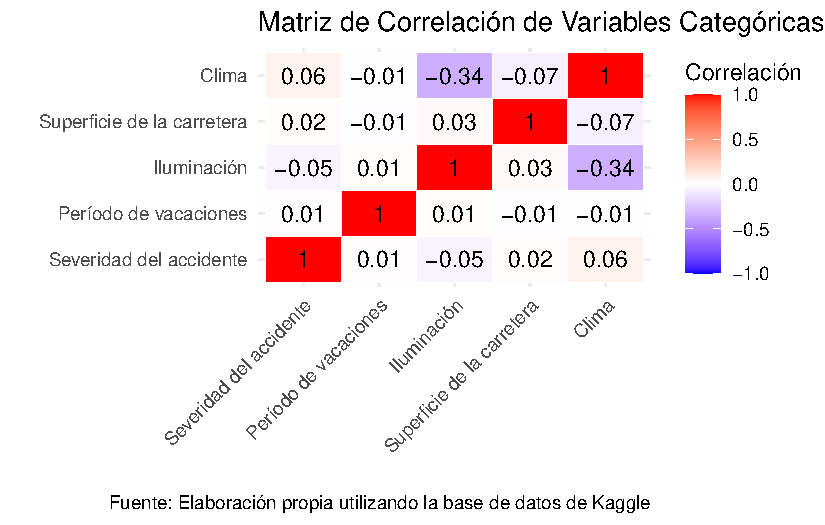
\includegraphics{cod_bitacora2_files/figure-pdf/unnamed-chunk-5-1.pdf}

Lo anterior se hizo con el fin de tener una \textbf{idea exploratoria
general} de cómo se mueven juntas las categorías al ser codificadas,
pero \textbf{esta correlación no debe interpretarse literalmente}, salvo
que las variables tengan un orden real y bien definido, de manera que lo
mejor para analizar independecia de variables categoricas son las
\textbf{tablas de contingencia} junto con \textbf{estadísticos como el
chi-cuadrado.}

Ahora, procederemos a construir una \textbf{matriz de correlación para
las variables numéricas} presentes en la base de datos. El propósito de
este análisis es evaluar la \textbf{relación lineal entre pares de
variables cuantitativas}, tales como la velocidad recomendada, el límite
de velocidad, el número de víctimas fatales, y las lesiones menores o
graves asociadas a los accidentes.

A diferencia de las variables categóricas, las variables numéricas
permiten calcular coeficientes de correlación como el
\textbf{coeficiente de Pearson}, que mide la \textbf{intensidad} de la
relación lineal entre dos variables. Un valor cercano a 1 indica una
fuerte correlación positiva, mientras que valores cercanos a -1 reflejan
una correlación negativa fuerte. Valores próximos a 0 sugieren ausencia
de relación lineal.

\begin{Shaded}
\begin{Highlighting}[]
\FunctionTok{library}\NormalTok{(ggplot2)}
\FunctionTok{library}\NormalTok{(reshape2)}

\NormalTok{data\_correlacion\_numerica }\OtherTok{\textless{}{-}}\NormalTok{ data }\SpecialCharTok{\%\textgreater{}\%}
  \FunctionTok{select}\NormalTok{(velocidad\_recomendada, fatales, lesiones\_menores, lesiones\_graves, limite\_velocidad)}


\FunctionTok{colnames}\NormalTok{(data\_correlacion\_numerica) }\OtherTok{\textless{}{-}} \FunctionTok{c}\NormalTok{(}
  \StringTok{"Velocidad recomendada"}\NormalTok{, }\StringTok{"Víctimas fatales"}\NormalTok{, }\StringTok{"Víctimas con lesiones menores"}\NormalTok{, }\StringTok{"Víctimas con lesiones graves"}\NormalTok{, }\StringTok{"Límite de velocidad"}
\NormalTok{)}

\CommentTok{\# Calcular la matriz de correlación}
\NormalTok{matriz\_correlacion\_numericas }\OtherTok{\textless{}{-}} \FunctionTok{cor}\NormalTok{(data\_correlacion\_numerica, }\AttributeTok{use =} \StringTok{"complete.obs"}\NormalTok{, }\AttributeTok{method =} \StringTok{"pearson"}\NormalTok{)}
\NormalTok{base\_matriz\_numericas }\OtherTok{\textless{}{-}} \FunctionTok{melt}\NormalTok{(matriz\_correlacion\_numericas)}

\CommentTok{\# Crear gráfico de calor con etiquetas numéricas}
\FunctionTok{ggplot}\NormalTok{(base\_matriz\_numericas, }\FunctionTok{aes}\NormalTok{(Var1, Var2, }\AttributeTok{fill =}\NormalTok{ value)) }\SpecialCharTok{+}
  \FunctionTok{geom\_tile}\NormalTok{(}\AttributeTok{color =} \StringTok{"white"}\NormalTok{) }\SpecialCharTok{+}
  \FunctionTok{geom\_text}\NormalTok{(}\FunctionTok{aes}\NormalTok{(}\AttributeTok{label =} \FunctionTok{round}\NormalTok{(value, }\DecValTok{2}\NormalTok{)), }\AttributeTok{size =} \DecValTok{4}\NormalTok{, }\AttributeTok{color =} \StringTok{"black"}\NormalTok{) }\SpecialCharTok{+}
  \FunctionTok{scale\_fill\_gradient2}\NormalTok{(}
    \AttributeTok{low =} \StringTok{"blue"}\NormalTok{, }\AttributeTok{mid =} \StringTok{"white"}\NormalTok{, }\AttributeTok{high =} \StringTok{"red"}\NormalTok{,}
    \AttributeTok{midpoint =} \DecValTok{0}\NormalTok{, }\AttributeTok{limit =} \FunctionTok{c}\NormalTok{(}\SpecialCharTok{{-}}\DecValTok{1}\NormalTok{, }\DecValTok{1}\NormalTok{), }\AttributeTok{space =} \StringTok{"Lab"}\NormalTok{, }\AttributeTok{name =} \StringTok{"Correlación"}
\NormalTok{  ) }\SpecialCharTok{+}
  \FunctionTok{theme\_minimal}\NormalTok{() }\SpecialCharTok{+}
  \FunctionTok{labs}\NormalTok{(}
    \AttributeTok{title =} \StringTok{"Matriz de Correlación de Variables Numéricas"}\NormalTok{,}
    \AttributeTok{x =} \StringTok{""}\NormalTok{, }\AttributeTok{y =} \StringTok{""}\NormalTok{,}
    \AttributeTok{caption =} \StringTok{"Fuente: Elaboración propia utilizando la base de datos de Kaggle"}
\NormalTok{  ) }\SpecialCharTok{+}
  \FunctionTok{theme}\NormalTok{(}
    \AttributeTok{axis.text.x =} \FunctionTok{element\_text}\NormalTok{(}\AttributeTok{angle =} \DecValTok{45}\NormalTok{, }\AttributeTok{hjust =} \DecValTok{1}\NormalTok{),}
    \AttributeTok{axis.text.y =} \FunctionTok{element\_text}\NormalTok{(}\AttributeTok{angle =} \DecValTok{0}\NormalTok{)}
\NormalTok{  )}
\end{Highlighting}
\end{Shaded}

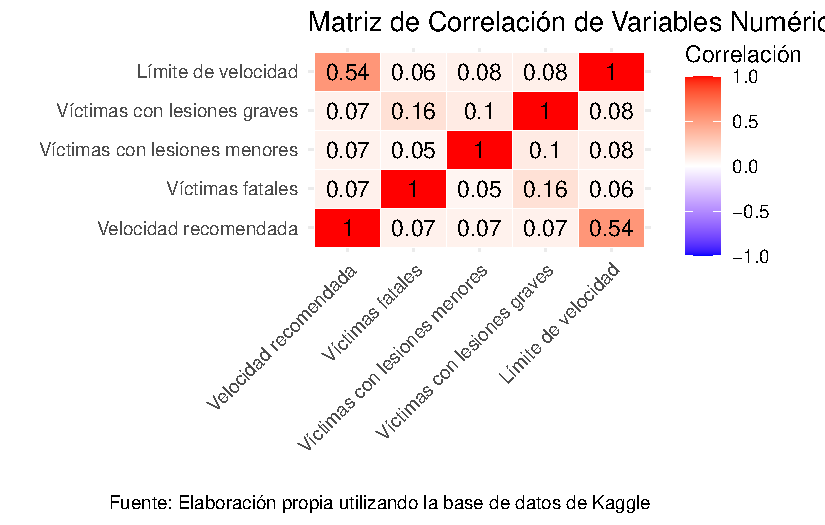
\includegraphics{cod_bitacora2_files/figure-pdf/unnamed-chunk-6-1.pdf}

Al analizar la matriz de correlación de las variables numéricas, se
observa una fuerte correlación positiva entre la velocidad recomendada y
el límite de velocidad, lo cual resulta intuitivo, dado que ambas están
directamente relacionadas con las condiciones del camino y las
normativas de tránsito. Esta relación indica que a medida que el límite
de velocidad aumenta en una determinada zona, también tiende a
incrementarse la velocidad recomendada para los conductores, lo que
podría refleja una adaptación de la infraestructura vial a las
condiciones del entorno, como el tipo de carretera y su capacidad de
soportar vehículos a mayor velocidad.

Por otro lado, se detecta una débil correlación entre el número de
víctimas fatales y las victímas con lesiones graves sugiere que, aunque
ambas variables están relacionadas con la severidad de los accidentes,
no necesariamente ocurren juntas de forma proporcional. Es decir, un
accidente con muchas lesiones graves no implica automáticamente la
presencia de víctimas fatales, y viceversa. Esta baja correlación puede
deberse a diversos factores, como la rapidez con que se presenta
asistencia médica, el tipo de accidente o el uso de medidas de seguridad
como cinturones.

Ahora daremos inicio al análisis gráfico de nuestra base de datos.
Comenzaremos explorando la distribución de la severidad de los
accidentes, una variable categórica fundamental en nuestro estudio. Dado
su carácter cualitativo, la forma más adecuada de visualizar esta
información es mediante un gráfico de barras, el cual nos permitirá
observar claramente la frecuencia de cada categoría de severidad
presente en el conjunto de datos. Esta representación facilitará la
identificación de patrones o posibles desequilibrios en la ocurrencia de
accidentes según su gravedad.

\begin{Shaded}
\begin{Highlighting}[]
\FunctionTok{library}\NormalTok{(ggplot2) }
\CommentTok{\# Gráfico con las distribuciones del género }

\FunctionTok{ggplot}\NormalTok{(data, }\FunctionTok{aes}\NormalTok{(}\AttributeTok{x =}\NormalTok{ severidad, }\AttributeTok{fill =}\NormalTok{ severidad)) }\SpecialCharTok{+} \FunctionTok{geom\_bar}\NormalTok{() }\SpecialCharTok{+} \FunctionTok{scale\_fill\_manual}\NormalTok{(}\AttributeTok{values =} \FunctionTok{c}\NormalTok{(}\StringTok{"Accidente fatal"} \OtherTok{=} \StringTok{"purple"}\NormalTok{, }\StringTok{"Accidente serio"} \OtherTok{=} \StringTok{"red"}\NormalTok{, }\StringTok{"Accidente leve"} \OtherTok{=} \StringTok{"blue"}\NormalTok{, }\StringTok{"Accidente sin lesiones"} \OtherTok{=} \StringTok{\textquotesingle{}gray\textquotesingle{}}\NormalTok{)) }\SpecialCharTok{+} \FunctionTok{labs}\NormalTok{(}\AttributeTok{x =} \StringTok{"Distribución de la Severidad de los Accidentes"}\NormalTok{, }\AttributeTok{y =} \StringTok{"Frecuencia"}\NormalTok{) }\SpecialCharTok{+} \FunctionTok{theme\_minimal}\NormalTok{() }\SpecialCharTok{+} \FunctionTok{labs}\NormalTok{(}\AttributeTok{caption =} \StringTok{"Fuente: Elaboración propia utilizando la base de datos de Kaggle"}\NormalTok{) }\SpecialCharTok{+} \FunctionTok{theme}\NormalTok{(}\AttributeTok{plot.caption =} \FunctionTok{element\_text}\NormalTok{(}\AttributeTok{hjust =} \FloatTok{0.5}\NormalTok{))}
\end{Highlighting}
\end{Shaded}

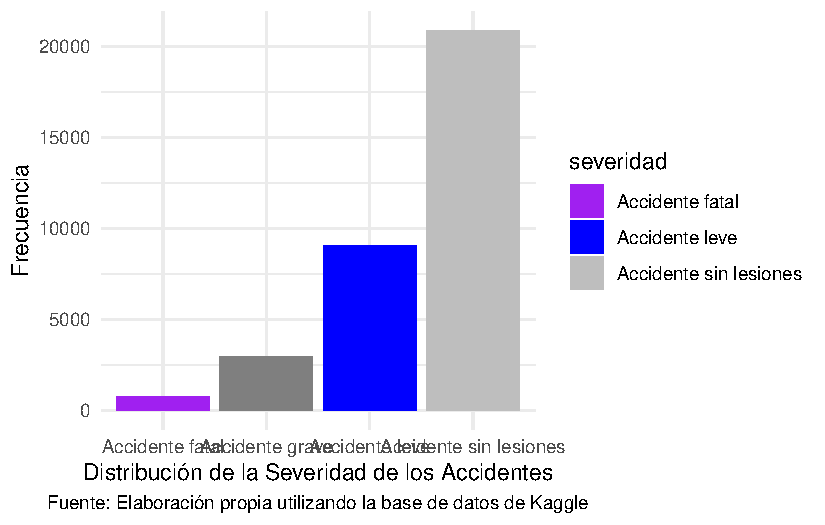
\includegraphics{cod_bitacora2_files/figure-pdf/unnamed-chunk-7-1.pdf}

El gráfico de barras revela que la mayoría de los accidentes registrados
en la base de datos corresponden a incidentes de severidad \textbf{leve
o sin heridos}, mientras que los casos más graves, como aquellos con
víctimas \textbf{serias o fatales}, son considerablemente menos
frecuentes. Esta distribución sugiere que, aunque los accidentes son
relativamente comunes, la mayoría no resultan en consecuencias
extremadamente severas. Sin embargo, la presencia, aunque baja, de
accidentes fatales resalta la importancia de seguir analizando los
factores asociados a estos casos críticos.

Además decidimos realizar un facet en esta misma variable con respecto a
la variable ``Education Level'', con el fin de visualizar la
distribución en cada categoría, esto porque queremos descartar o validar
que de alguna forma el nivel educativo tiene relación con nuestra
variable objetivo, la cual es la calificación de riesgo.

\begin{Shaded}
\begin{Highlighting}[]
\FunctionTok{library}\NormalTok{(ggplot2)}
\FunctionTok{library}\NormalTok{(dplyr)}


\FunctionTok{ggplot}\NormalTok{(data, }\FunctionTok{aes}\NormalTok{(}\AttributeTok{x =}\NormalTok{ clima, }\AttributeTok{fill =}\NormalTok{ severidad)) }\SpecialCharTok{+}
  \FunctionTok{geom\_bar}\NormalTok{(}\AttributeTok{position =} \StringTok{"fill"}\NormalTok{) }\SpecialCharTok{+} 
  \FunctionTok{labs}\NormalTok{(}
    \AttributeTok{title =} \StringTok{"Distribución de la Severidad de los Accidentes según el Clima"}\NormalTok{,}
    \AttributeTok{x =} \StringTok{"Condiciones Climáticas"}\NormalTok{,}
    \AttributeTok{y =} \StringTok{"Proporción"}\NormalTok{,}
    \AttributeTok{fill =} \StringTok{"Severidad"}
\NormalTok{  ) }\SpecialCharTok{+}
  \FunctionTok{theme\_minimal}\NormalTok{() }\SpecialCharTok{+}
  \FunctionTok{scale\_fill\_manual}\NormalTok{(}\AttributeTok{values =} \FunctionTok{c}\NormalTok{(}
    \StringTok{"Accidente fatal"} \OtherTok{=} \StringTok{"\#990000"}\NormalTok{,        }\CommentTok{\# rojo oscuro}
    \StringTok{"Accidente grave"} \OtherTok{=} \StringTok{"\#cc0000"}\NormalTok{,      }\CommentTok{\# rojo intermedio}
    \StringTok{"Accidente leve"} \OtherTok{=} \StringTok{"\#e06666"}\NormalTok{,        }\CommentTok{\# rojo más claro}
    \StringTok{"Accidente sin lesiones"} \OtherTok{=} \StringTok{"\#f4cccc"}    \CommentTok{\# rojo muy claro}
\NormalTok{  ))}
\end{Highlighting}
\end{Shaded}

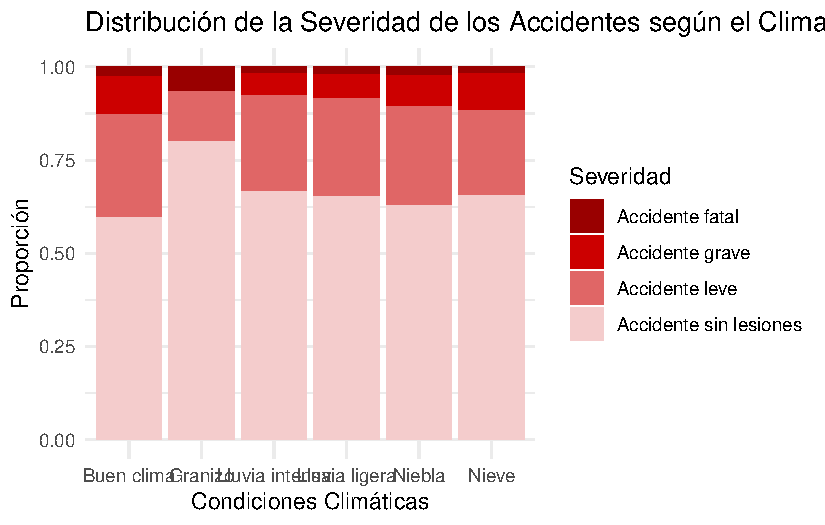
\includegraphics{cod_bitacora2_files/figure-pdf/unnamed-chunk-8-1.pdf}




\end{document}
